\chapter{Results}
\label{chapter:results}

\section{Applications Based on the DDE framework}
\label{sec:result-applications}
  To test the throughput of messages, scalability of the framework and round trip time of message delivery, two sample applications were created based on the DDE framework. The sample applications described in \autoref{subsec:producer-consumer-program} and
  \autoref{sec:request-reply-program} were used for testing and evaluation of the framework.

\subsection{Producer/Consumer Program}
\label{subsec:producer-consumer-program}
  The producer-consumer program is a simple application. It has two worker isolates, a producer and a consumer. The ‘producer’, shown in \autoref{lst:producer}, starts producing 64-byte messages as soon as it is spawned. The ‘producer’ worker continues producing messages until it is terminated. The produced messages are targeted for the ‘consumer’~[\autoref{lst:consumer}] worker which is done by setting the target address of the consumer to “mysystem/consumer” as the second argument of \emph{send()} (line 31). Here, the first part of the address “mysystem” is the name of the isolate system where the ‘consumer’ worker is supposed to be deployed.

  The ‘consumer’ worker shown in \autoref{lst:consumer} dequeues a message from its queue as soon as it is spawned.  After receiving each message, the consumer prints it to standard output and invokes \emph{done()} which sends a dequeue request to fetch another message.

\newpage
\begin{lstlisting}[language=java, firstnumber=1, caption=Basic version of Producer Worker of Producer-Consumer application, label=lst:producer]
import 'dart:io';
import 'dart:isolate';
import 'dart:async';
import 'dart:math' as Math;
import 'package:isolatesystem/worker/Worker.dart';

main(List<String> args, SendPort sendPort) {
  Producer producer = new Producer(args, sendPort);
}

class Producer extends Worker {
  static const String consumerAddress = "mysystem/consumer";
  static const String Message64Bytes = "012345670123456701234567";

  StringBuffer data = new StringBuffer();

  Producer(List<String> args, SendPort sendPort) : super(args, sendPort) {
    description += "${args}";
    sendMsgWithDelay();
  }

  @override
  onReceive(message) {}

  sendMsgWithDelay() {
    while(true) {
      int timestamp = new DateTime.now().millisecondsSinceEpoch;
      Map message = {'createdAt': timestamp, 'message': Message64Bytes};
      int delay = 20 + new Math.Random().nextInt(480);
      sleep(new Duration(microseconds:delay));
      send(message, consumerAddress);
    }
  }
}
\end{lstlisting}


% Consumer Worker
\newpage
\begin{lstlisting}[language=java, firstnumber=1, caption=Basic version of Consumer Worker of Producer-Consumer application, label=lst:consumer]
  import 'dart:isolate';
  import 'package:isolatesystem/worker/Worker.dart';

  main(List<String> args, SendPort sendPort) {
    Consumer printerIsolate = new Consumer(args, sendPort);
  }

  class Consumer extends Worker {
    Consumer(List<String> args, SendPort sendPort) : super(args, sendPort);

    @override
    onReceive(message) {
      outText(message);
    }

    outText(var message) {
      print(message);
      done();
    }
  }

\end{lstlisting}

\subsection{Requester/Supplier Program}
\label{sec:request-reply-program}
The request-reply program is a simple application. It has two worker isolates, a requester and a supplier. The ‘requester’ shown in \autoref{lst:requester} sends a request message as soon as it is spawned. It randomly generates a request for a fruit, a number or a name. This request message is targeted for the ‘supplier’~[\autoref{lst:consumer}] worker by setting its address as the second argument of \emph{ask()}.

  The ‘supplier’ worker shown in \autoref{lst:consumer} does a pattern matching on each request and based on the request message, it either replies with a random fruit, a random number or a random name to the original requester.

\newpage
% Requester Worker
\begin{lstlisting}[language=java, firstnumber=1, caption=Requester Worker of Requester-Supplier application, label=lst:requester]
import 'dart:isolate';
import 'dart:math';
import 'package:isolatesystem/worker/Worker.dart';
import 'AvailableSupplies.dart';

main(List<String> args, SendPort sendPort) {
  new Requester(args, sendPort);
}

class Requester extends Worker {
  static const String SupplierAddress = "demosystem/supplier";
  DateTime startTime;

  Requester(List<String> args, SendPort sendPort):super(args, sendPort) {
    startTime = new DateTime.now();
    _sendRequest();
  }

  @override
  onReceive(message) {
    int receivedAt = new DateTime.now().millisecondsSinceEpoch;
    int requestedAt = message['requestedAt'];
    int repliedAt = message['repliedAt'];
    int rtt = receivedAt - requestedAt;
    print("Round trip time: $rtt");
    _sendRequest();
  }

  _sendRequest() {
    String requestMessage = "";
    int randomNumber = new Random().nextInt(3);
    if(randomNumber == 1) {
      requestMessage = AvailableSupplies.RANDOM_FRUIT;
    } else if (randomNumber == 2) {
      requestMessage = AvailableSupplies.RANDOM_NUMBER;
    } else {
      requestMessage = AvailableSupplies.RANDOM_NAME;
    }

    Map message = {'requestedAt':new DateTime.now().millisecondsSinceEpoch, 'requestMessage':requestMessage};
    ask(message, SupplierAddress);
  }
}

\end{lstlisting}

% Supplier Worker
\begin{lstlisting}[language=java, firstnumber=1, caption=Requester Worker of Requester-Supplier application, label=lst:supplier]

import 'dart:isolate';
import 'dart:math';
import 'package:isolatesystem/worker/Worker.dart';
import 'AvailableSupplies.dart';

main(List<String> args, SendPort sendPort) {
  new Supplier(args, sendPort);
}

class Supplier extends Worker {
  Supplier(List<String> args, SendPort sendPort):super(args, sendPort);

  @override
  onReceive(message) {
    String responseMessage = "";
    switch(message['requestMessage']) {
      case AvailableSupplies.RANDOM_FRUIT:
        responseMessage = _randomFruit();
        break;
      case AvailableSupplies.RANDOM_NUMBER:
        responseMessage = _randomNumber();
        break;
      case AvailableSupplies.RANDOM_NAME:
        responseMessage = _randomName();
        break;
    }
    Map response = {
        'requestedAt': message['requestedAt'],
        'repliedAt': new DateTime.now().millisecondsSinceEpoch,
        'requestMessage': message['requestMessage'],
        'responseMessage': responseMessage};
    reply(response);
    done();
  }

  String _randomFruit() {
    int number = new Random().nextInt(5);
    return ["APPLE", "ORANGE", "KIWI", "PEAR", "GRAPES"][number];
  }

  String _randomNumber() {
    return new Random().nextInt(99999).toString();
  }

  String _randomName() {
    int number = new Random().nextInt(5);
    return ["Lorna", "Ambrose", "Domingo", "Kirsten", "Zachery"][number];
  }
}

\end{lstlisting}

% Supporting Class
\begin{lstlisting}[language=java, firstnumber=1, caption=Supporting class that contains list of constants for pattern matching, label=lst:supportingClass]

class AvailableSupplies {
  static const String RANDOM_FRUIT = "supply.fruit";
  static const String RANDOM_NUMBER = "supply.number";
  static const String RANDOM_NAME = "supply.name";
}
\end{lstlisting}


\subsection{System Setup for Testing}
    The benchmarks of the sample applications were performed in Amazon EC2~\footnote{\url{http://aws.amazon.com/ec2}} instances. A distributed environment with configurations shown in \autoref{tab:specs} was setup on multiple EC2 instances.

\begin{table}[H]
  \caption[Specification of machines used for testing and benchmarking]{Specification of machines used for testing and benchmarking}\label{tab:specs}
  \centering
  \begin{tabular}{l l l}
    \toprule
      \bf{Deployed Systems} & \bf{Name} &  \bf{Specifications}\\
    \midrule

      \pbox{30cm}{\relax RabbitMQ and\\a Message Queuing System} & c3.2xLarge & \pbox{60cm}{8 core CPU, 28 ECU,\\15 GiB Memory, SSD disk}\\
\midrule
      \pbox{30cm}{\relax Message Queuing System} & m3.2xLarge & \pbox{60cm}{8 core CPU, 26 ECU,\\30 GiB Memory, SSD disk}\\
\midrule
      \pbox{20cm}{\relax Registry and\\File Server} & m3.xLarge & \pbox{60cm}{2 core CPU, 13 ECU,\\15 GiB Memory, SSD disk}\\
\midrule
      \pbox{20cm}{\relax Isolate Systems (Nodes)} & m3.xLarge & \pbox{60cm}{2 core CPU, 13 ECU,\\15 GiB Memory, SSD disk}\\

    \bottomrule
  \end{tabular}
\end{table}

\subsection{Observations From DDE Based Applications}
\label{subsec:result-framework}
   Some observations made during the development and the deployment of applications based on the DDE framework were:

\begin{itemize}
  \item The program source code based on the DDE framework is short, as evident from the source code of the applications listed in \autoref{sec:result-applications}.

  \item The worker isolate could not be run in a browser because of current limitations of the Dart VM.

  \item Setting up the system for the first time was complicated because it consisted of several components that needed to be started up separately.

  \item Once the system was setup, adding workers and isolate systems to the nodes was easy. Thus, deploying an application to a distributed system was easy.

  \item Shutting down a single isolate or an isolate system did not effect other components and nodes.

  \item The decoupling of isolate systems, the MQS and the registry allowed each component to start up and shutdown without severely affecting other systems.

  \item The worker isolates developed for an application were loosely coupled. They were coupled only in terms of messages.
  % But, the sender needed to know address of a target worker isolate, which depend on deployment. Thus one more coupling ! This can be future improvement.

  \item The REST API exposed by the registry simplified the deployment of isolate systems to different nodes.

  \item The Web interface of the Registry provided the ability to visualize and monitor the cluster.

  \item Messages sent to RabbitMQ were not lost during the restart of the system because they were persisted in RabbitMQ. The system continued to process messages after the restart.
\end{itemize}

\section{Benchmarks}
\label{sec:benchmarks}
  The benchmarks discussed here are the results of the evaluation of applications discussed in~\autoref{sec:result-applications}. The results presented in this chapter were performed on Amazon EC2 servers\footnote{EC2 servers of data center in Ireland} with configurations shown in table~\autoref{tab:specs}

\subsection{Production Throughput of Isolates}
  % In contrast to results of production throughput of messages as seen in \autoref{fig:result-productionMessageSize} and \autoref{fig:result-productionRabbit},
  The result shown in
 \autoref{fig:result-productionIsolate} is the throughput of message production by the isolate system before the messages are sent to the MQS and broker for enqueuing. The production of a message in a worker isolate was throttled, so that there is no immediate ‘out of memory’ error from an overwhelming production of messages. Throughput was throttled by delaying the production of messages by a random amount of time ranging from 20~-~500 microseconds. The observations made here are the average throughput of each worker isolate as well as average throughput of all the producer nodes connecting to a single MQS instance.

  As observed in the \autoref{fig:result-productionIsolate}, the total production rate of messages sharply increased when increasing the number of producers. In contrast, the average production of a single node was lower with a higher number of producers.

  In Dart version 1.7.2, time required to send a message of ‘Map’ datatype from one isolate to another consumed around 300~-~500 microseconds. But, when the same message was serialized to JSON String the time required to send a message dropped to 10~-~40 microseconds. It is an improvement in speed by one order of magnitude.

\begin{figure}[H]
  \centering  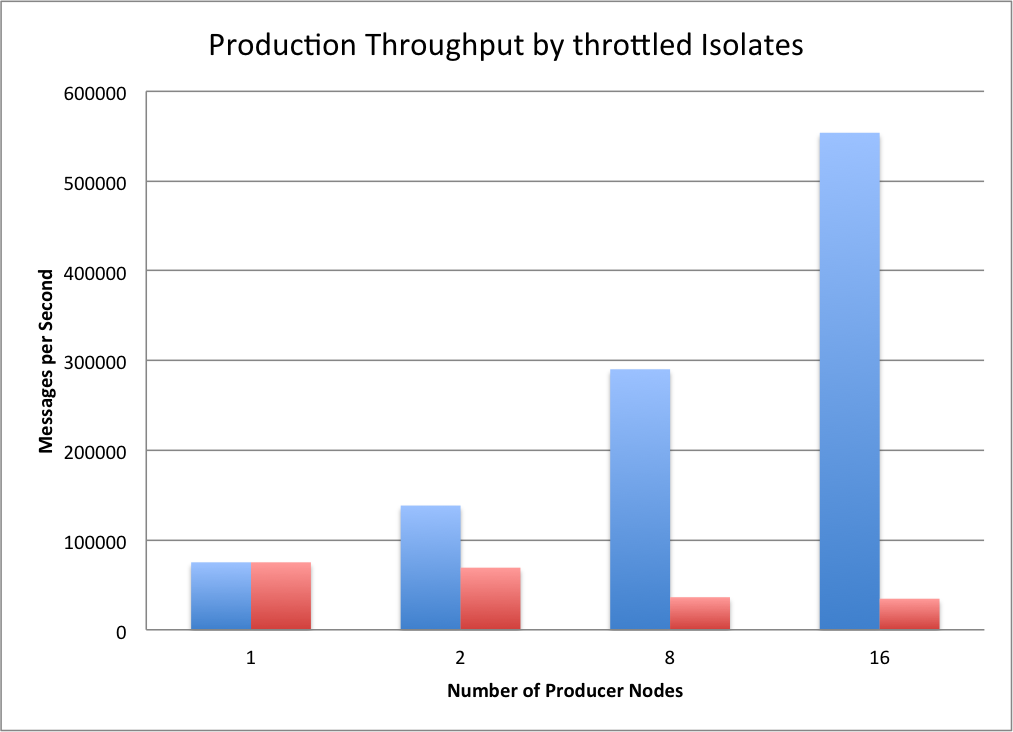
\includegraphics[width=1\textwidth]{figures/06productionIsolate}
  \caption[Production Throughput of Isolate]{Production Throughput of Isolate}
  \label{fig:result-productionIsolate}
\end{figure}

\subsection{Message Size}
\label{subsec:messageSize}
The result shown in \autoref{fig:result-consumptionMessageSize} was obtained by having eight consumers with a prefetch count of 8 to dequeue existing messages from a queue.

  The negative effect on message consumption throughput of larger messages is evident from \autoref{fig:result-consumptionMessageSize}. The decrease with message throughput was more prominent between message sizes of 256 bytes and 512 bytes than that of between 64 bytes and 256 bytes.

  Similar observation can be made from~\autoref{fig:result-productionMessageSize} which is a result of allowing a single worker isolate to create messages, except there was a slight rise in the throughput when the message size was increase from 512 bytes to 1024 bytes.

\begin{figure}[H]
  \centering  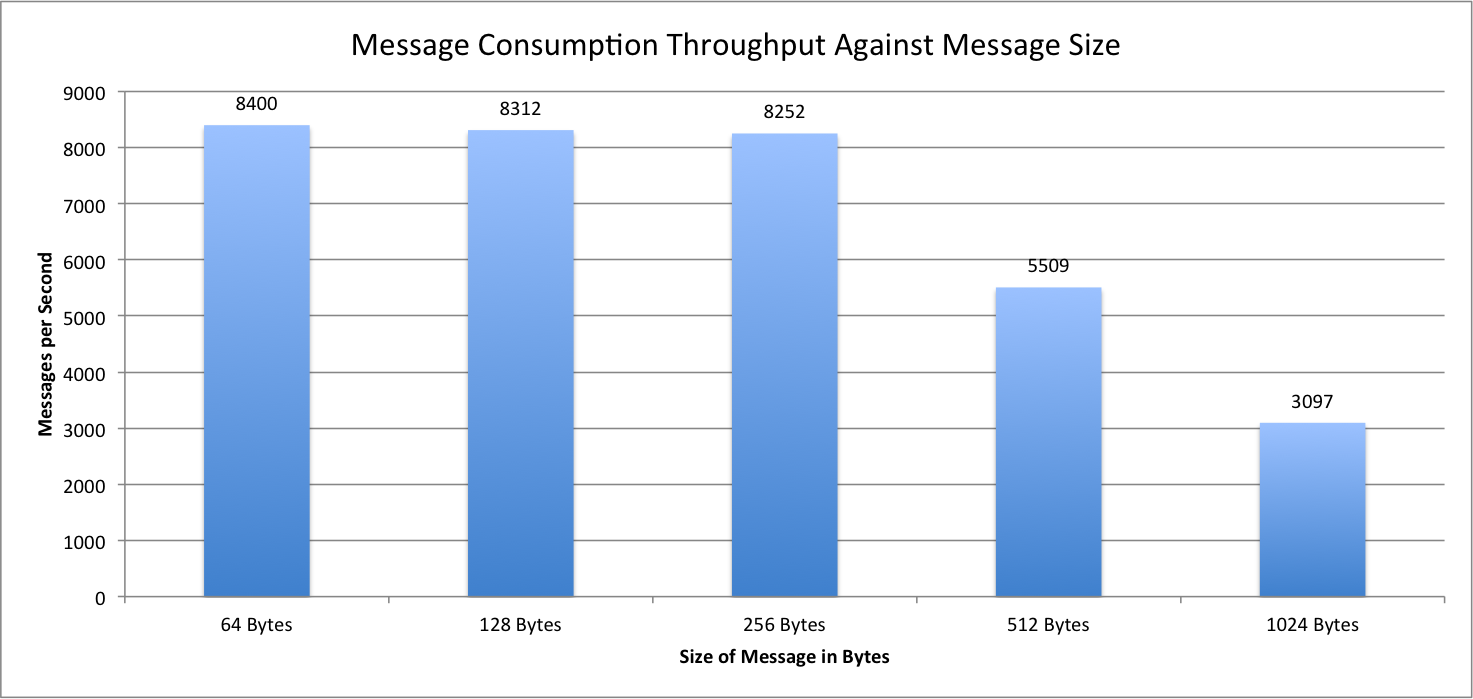
\includegraphics[width=1\textwidth]{figures/02consumptionMessageSize}
  \caption[Message Consumption Throughput vs Message Size]{Message Consumption Throughput vs Message Size (Higher is better)}
  \label{fig:result-consumptionMessageSize}
\end{figure}

\begin{figure}[H]
  \centering  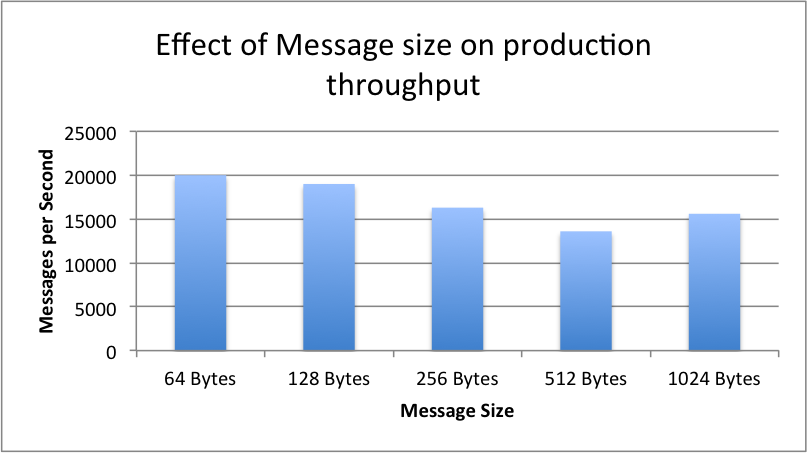
\includegraphics[width=0.8\textwidth]{figures/03productionMessageSize}
  \caption[Message Production Throughput vs Message Size]{Message Production Throughput vs Message Size (Higher is better)}
  \label{fig:result-productionMessageSize}
\end{figure}

\subsection{Number of Message Queuing Systems}
  \autoref{fig:result-varyingMqs} is the result obtained by testing message consumption for 1 to 32 consumers distributed to one to four MQS instances connected to the same message broker. Adding MQS instances clearly increased message throughput. Nevertheless, adding more than eight consumers per MQS instance had a negative effect, as we can see from the decline of throughput in the line charts for the one-instance case and the two-instance case. In the tests with one and two MQS instances, the optimum performance was seen when there were 8 consumers in total. But with four MQS instances, the throughput kept rising and supported up to 32 consumers without decline in performance. Nevertheless, the rate of performance increase was not as much as the rate seen when scaling up from two MQS instances to four MQS instances.

  The positive impact of scaling out the MQS was seen not only on consumption throughput but also on production throughput. \autoref{fig:result-productionRabbit} shows results of message production throughput by increasing the number of producers from one to eight, distributed across multiple MQS instances. The production rate measured here was the rate at which RabbitMQ enqueued messages, not the rate at which a worker isolate produced messages.
\begin{figure}[H]
  \centering
  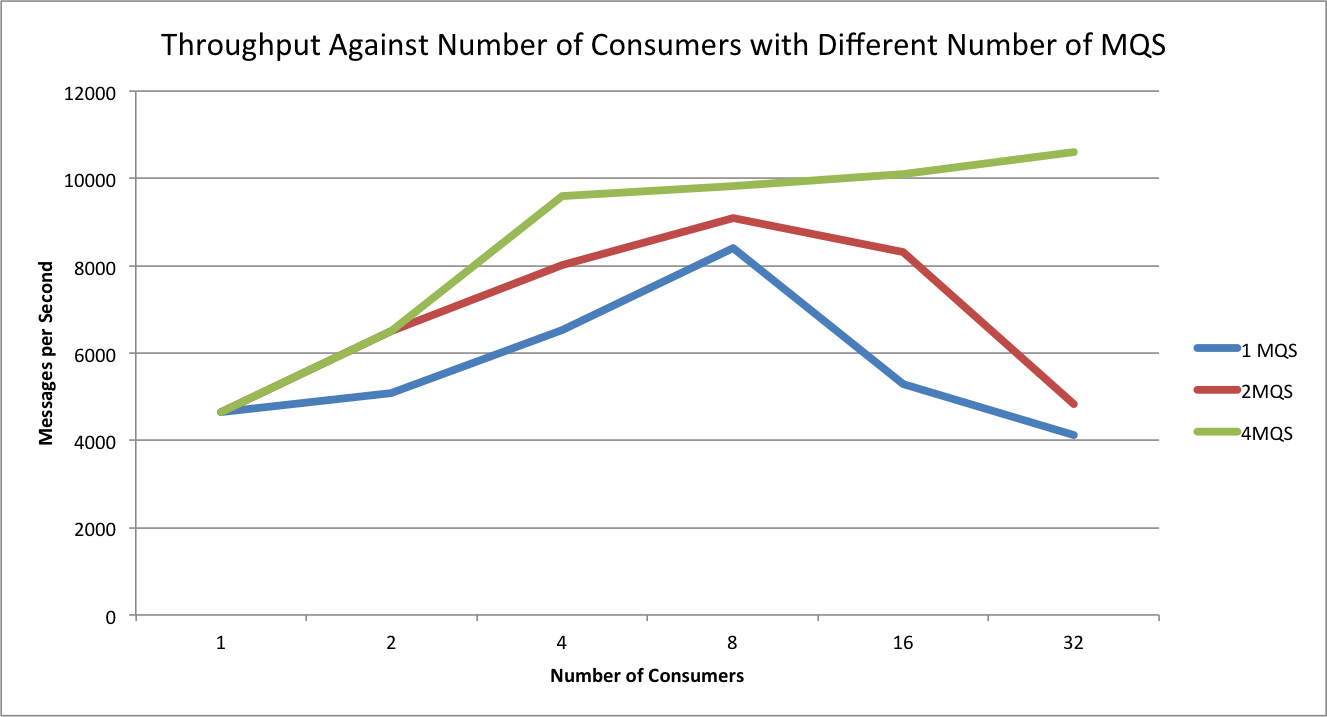
\includegraphics[width=1\textwidth]{figures/04varyingMqs}
  \caption[Consumption Throughput on Scaled out Message Queuing System]{Consumption Throughput on Scaled out Message Queuing System}
  \label{fig:result-varyingMqs}
\end{figure}


\begin{figure}[H]
  \centering  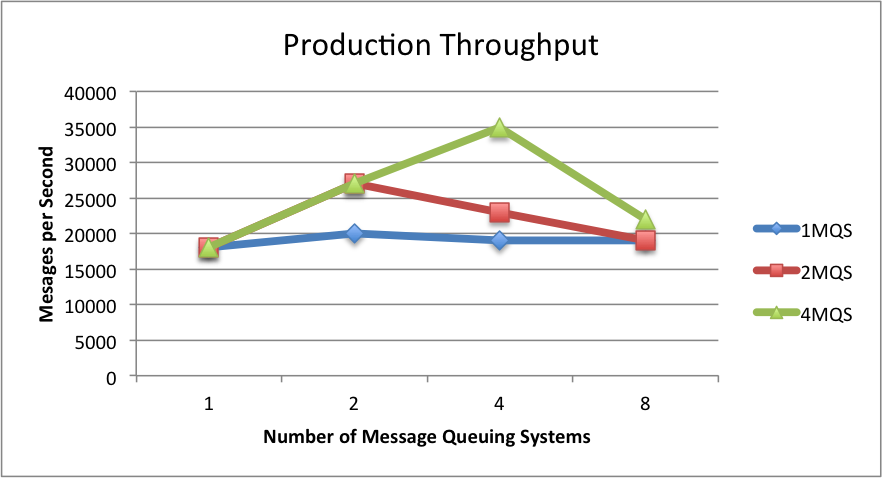
\includegraphics[width=0.9\textwidth]{figures/05productionRabbit}
  \caption[Production Throughput on Scaling out Message Queuing System]{Production Throughput on Scaling out Message Queuing System}
  \label{fig:result-productionRabbit}
\end{figure}

\subsection{Prefetch Count}
\label{subsec:prefetchCount}
\autoref{fig:result-prefetch} shows the variation in overall message consumption when the number of consumers (separate isolate systems in separate nodes) were increased. Each line in the figure represents different values for the prefetch-count~[\autoref{subsec:rabbitmqPrefetch}] value set by the consumer while subscribing to the message broker system. Depending upon prefetch-count, increase, peak and decline of message consumption throughput can be seen for different numbers of consumers.

  The increase in consumers had significant positive results for message throughput, but we can see that after around 8 consumers, adding more consumers had negative effect in the overall throughput.

    Increasing prefetch count had more positive impact in message throughput compared to increasing consumers. For instance, the increase in consumers from 1 to 16 resulted in the rise of approximately 2000 messages per second, while the increase in prefetch-count from 1 to 16 in the single consumer case resulted in an increase of message throughput by approximately 5500 messages per second.

\begin{figure}[H]
  \centering
  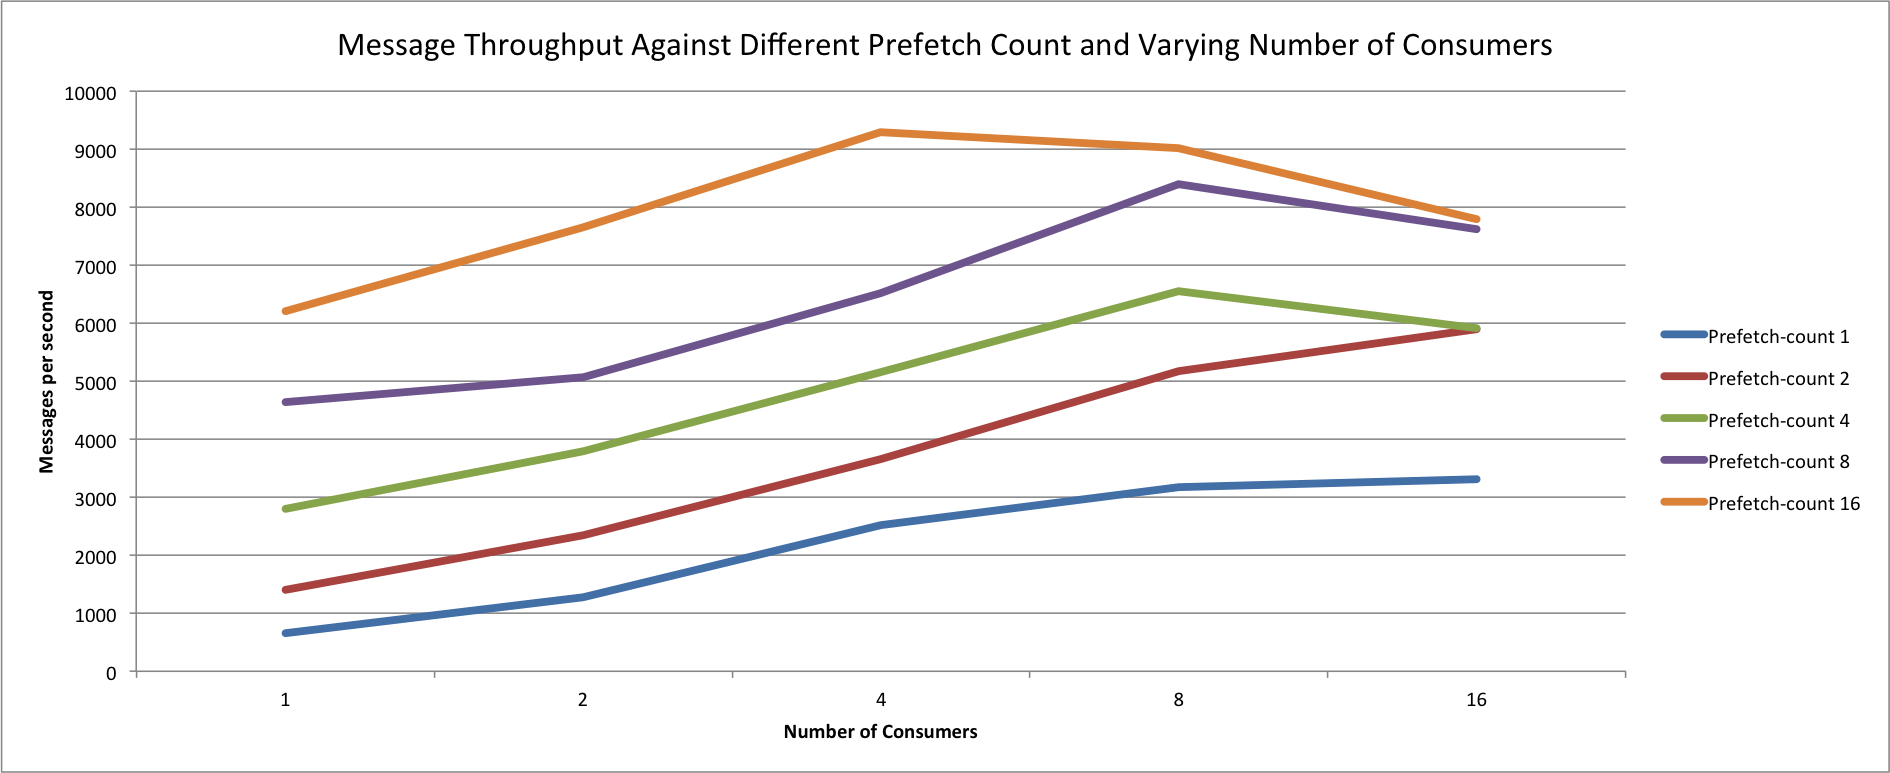
\includegraphics[width=1\textwidth]{figures/01prefetch}
  \caption[Message Throughput vs Number of consumers for varying prefetch-count]{Message Throughput vs Number of consumers for varying prefetch-count (Higher is better)}
  \label{fig:result-prefetch}
\end{figure}


\subsection{Simultaneous Production and Consumption}
\label{subsec:simultaneous}
  In contrast to previous benchmarks, which were measured with either only producers or only consumers, the benchmarks in \autoref{fig:result-simultaneous1} and \autoref{fig:result-simultaneous2} show the consumption rate and production rate of messages when producers and consumers are run simultaneously in different nodes. Compared to what was seen in \autoref{fig:result-prefetch} and
  \autoref{fig:result-varyingMqs}, the consumption rate is lower in this case. Nevertheless, the production rate of messages remained almost equal to that which was observed in \autoref{fig:result-varyingMqs} with a single MQS instance.

  If we compare \autoref{fig:result-simultaneous1} and \autoref{fig:result-simultaneous2}, scaling out with producers and consumers connecting to different MQS instances had a significant positive impact in overall message throughput. Especially, in this case the consumption rate increased by almost an order of magnitude than that of using a single MQS instance. A slight increase in production throughput was also observed with additional MQS instances.

\begin{figure}[H]
  \centering
  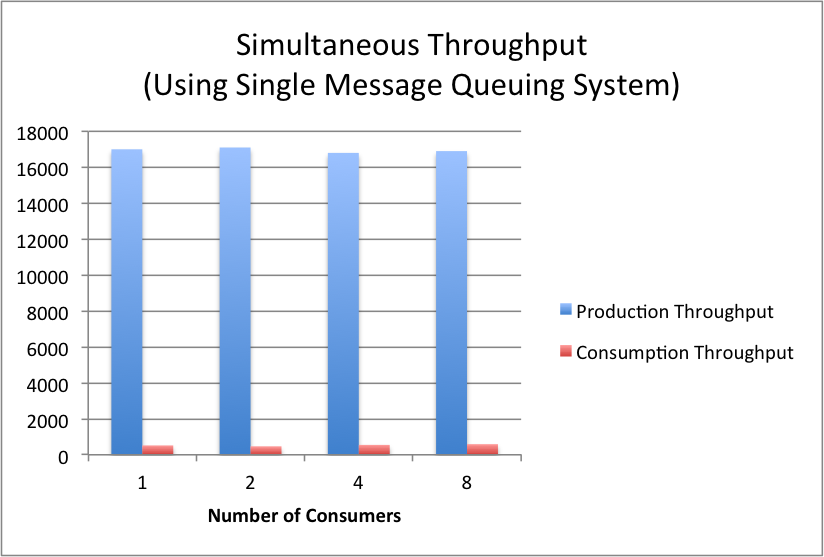
\includegraphics[width=0.8\textwidth]{figures/07simultaneous1}
  \caption[Throughput during simultaneous execution in single MQS]{Throughput during simultaneous execution in a single MQS instance}
  \label{fig:result-simultaneous1}
\end{figure}

\begin{figure}[H]
  \centering
  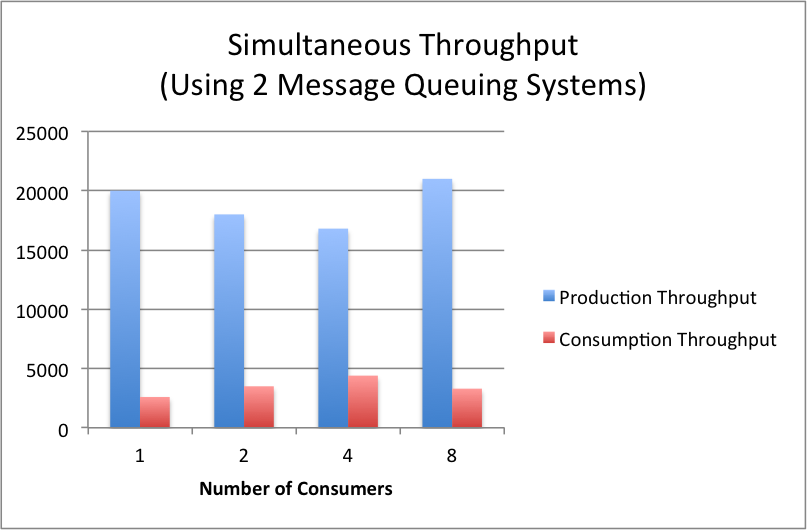
\includegraphics[width=0.8\textwidth]{figures/08simultaneous2}
  \caption[Throughput during simultaneous execution in two MQS]{Throughput during simultaneous execution in two MQS instances}
  \label{fig:result-simultaneous2}
\end{figure}


\subsection{Throughput of Request-Reply}
\label{subsec:request-reply}
  The request-reply application used for testing is different from the producer-consumer application in terms of how the messages are produced and consumed. In request-reply, a message is produced by the producer only when it receives a request from the requester (and the requester sends a request for another message only after it receives the reply) whereas, in the producer-consumer application the producer creates messages regardless of the existence of consumers. Also, in the producer-consumer application any instance of a target worker isolate of any node may consume the message as it is designated only by the name of the worker isolate. But in request-reply the reply message is sent to the worker isolate that originated the request.

  For single execution of a message in the producer-consumer application, the steps required are enqueuing the message from producer and then dequeuing the message by the consumer. Whereas, in case of request-reply, first a request message must be enqueued and dequeued, then the reply message must be enqueued and dequeued. Thus, the steps required in the request-reply case are twice as much as in the producer-consumer case.

  In \autoref{fig:result-request-reply}, when the number of consumers were increased we can see a linear increase in the production and consumption rate of messages. However, adding more suppliers had very little effect in overall throughput. The maximum increase in throughput by adding suppliers was seen when there were more consumers.
\begin{figure}[H]
  \centering
  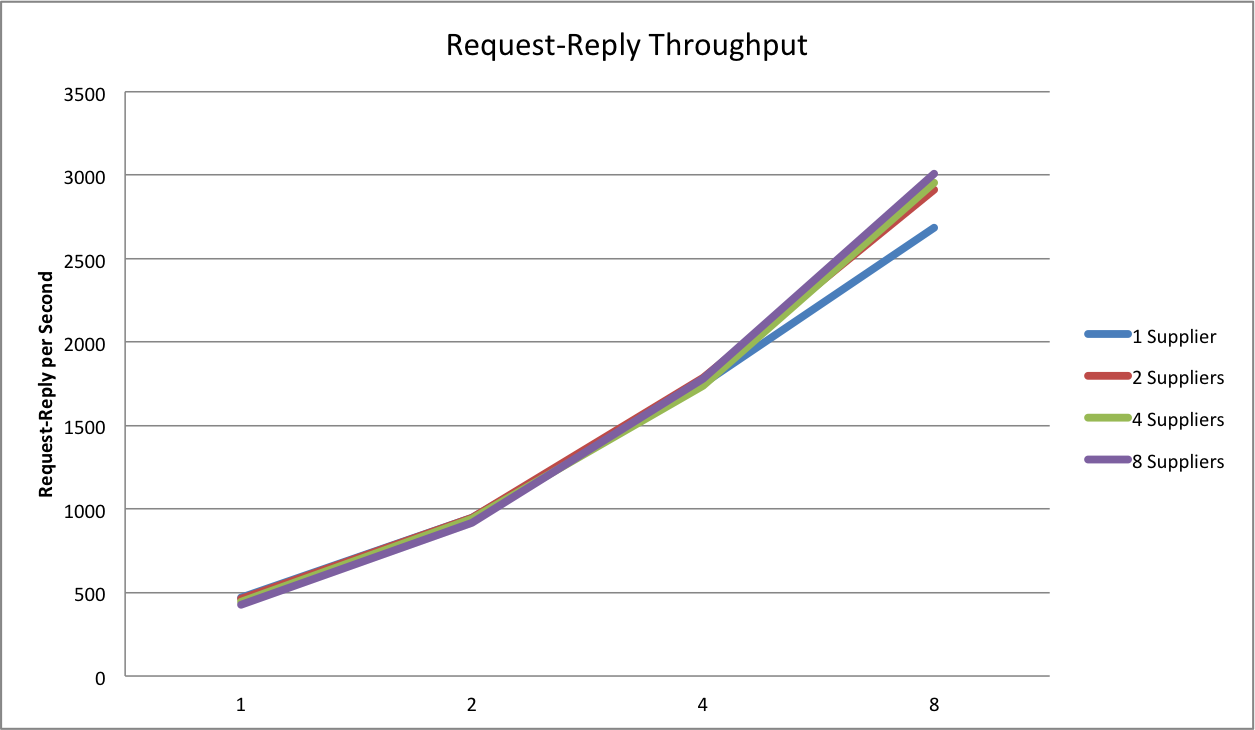
\includegraphics[width=0.85\textwidth]{figures/09request-reply}
  \caption[Throughput of request-reply]{Throughput of request-reply}
  \label{fig:result-request-reply}
\end{figure}

\subsection{Round Trip Time in Request-Reply}
\label{subsec:request-reply-rtt}
  The results seen in \autoref{fig:result-request-reply-rtt} are the benchmarks of average round trip time (RTT) of messages in the request-reply case.

  The result was obtained by attaching a timestamp in the message that was sent to the supplier; upon receiving the request message at the supplier, the timestamp was copied to the reply message and sent back to the sender (requester). The difference between the timestamp when the message was received at the requester and the timestamp contained in the message is the round trip time.

  From the result of RTT shown in \autoref{fig:result-request-reply-rtt}, we can see that there were inconsistencies in RTT of messages with respect to the number of suppliers and requesters. When there was only one supplier, the RTT of a message was usually higher compared to cases when there were more suppliers. Nevertheless, the least inconsistency was seen in the case of 8 suppliers and the least latency was observed in the case of a single supplier with a single consumer.

  \begin{figure}[H]
    \centering    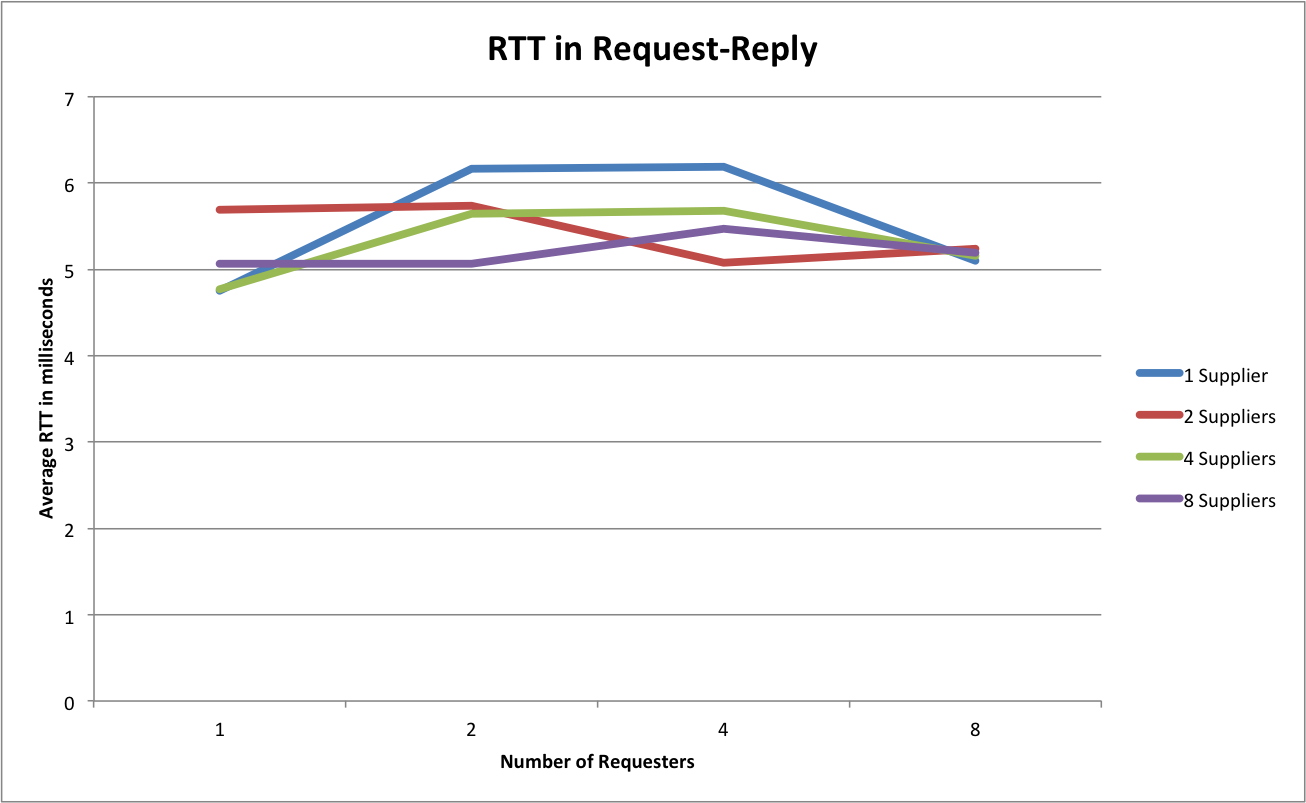
\includegraphics[width=0.85\textwidth]{figures/10request-reply-rtt}
    \caption[Round trip times of messages in request reply]{Round trip times of messages in request reply (Lower is better)}
    \label{fig:result-request-reply-rtt}
  \end{figure}
